\documentclass[a4paper]{article}

\usepackage[utf8]{inputenc}
\usepackage[T1]{fontenc}
\usepackage[english]{babel}

\usepackage{amsmath}
\usepackage{amssymb}
\usepackage{amsfonts}
\usepackage{amsthm}
\usepackage{dsfont}
\theoremstyle{plain}
\usepackage{xfrac}

\usepackage{listings}
\usepackage{mathtools}
\usepackage{color}

\definecolor{mygreen}{rgb}{0,0.6,0}
\definecolor{mygray}{rgb}{0.5,0.5,0.5}
\definecolor{mymauve}{rgb}{0.58,0,0.82}

\lstset{
  backgroundcolor=\color{white},
  basicstyle=\footnotesize,
  breakatwhitespace=false,
  breaklines=true,
  captionpos=b,
  commentstyle=\color{mygreen},
  deletekeywords={...},
  escapeinside={\%*}{*)},
  extendedchars=true,
  frame=none,
  keepspaces = true,
  keywordstyle=\color{blue},
  language=Python,
  otherkeywords={*,...},
  numbers=left,
  numbersep=5pt,
  numberstyle=\tiny\color{mygray},
  rulecolor=\color{black},
  showspaces=false,
  showstringspaces=false,
  showtabs=false,
  stepnumber=5,
  stringstyle=\color{mymauve},
  tabsize=2,
  title=\lstname
}

\usepackage{enumerate}
\usepackage[colorlinks=true]{hyperref}
\usepackage{graphicx}
\graphicspath{{figures/}} 
\usepackage[top=3cm, bottom=3cm, left=3cm, right=3cm]{geometry}
\usepackage{float}
\usepackage{wrapfig} % Allows wrapping text around tables and figures

\usepackage{caption}
\usepackage{subcaption}
\usepackage{booktabs} % Top and bottom rules for table

\usepackage{tikz}
\usetikzlibrary{arrows}

\usepackage[square,numbers]{natbib}

\title{\Huge Recidivism of Criminal Offenders \newline \LARGE A machine-learning approach to justice \newline {}}
\author{\textbf{Estienne Granet} \\
  Department of Statistics\\
  Harvard University \\
  \href{mailto:egranet@g.harvard.edu}{egranet@g.harvard.edu}
  \and
  \textbf{Victor Lei} \\
  Department of Computer Science\\
  Harvard University \\
  \href{mailto:vlei@g.harvard.edu}{vlei@g.harvard.edu}}

\date{\today}

\begin{document}

\maketitle

\begin{abstract}
Recidivism of criminal offenders is a difficult topic in criminal justice. If we view the justice system as serving an important rehabilitatory purpose, then recidivism represents indicators for potential improvement in the correctional system. Using a public data-set on two cohorts of inmates released from North Carolina prisons in 1978 and 1980, we build two predictors of whether an individual will offend again in the future. Our first predictor is one-layer feed-forward neural networks. The second predictor is random forest. Results are presented below.
\end{abstract}

\section*{Introduction}

Our goal is to effectively forecast whether an offender will offender again in the future when he or she is released from prison. To achieve this goal, we rely on a survey conducted on prisoners released from North Carolina prisons in 1978 and 1980. The survey contains information on the background of the offenders, including their involvement in drugs or alcohol, level of schooling, nature of the crime resulting in the sample conviction, number of prior incarcerations and recidivism during the followup period following release from the sample
incarceration. The dataset also contains information on the
the marital status, the sex, the age and the race of the offenders. In hard numbers, the dataset contains 9,327 profiles for prisoners released in 1978 and 9,549 profiles for prisoners released in 1980. Each entry has 16 variables and most variables are indicators. In order to be consistent with the dataset used in previous work, we process the dataset by removing all defective entries (130 from each dataset) and all entries with missing values (4,709 from the 1978 data and 3,810 from the 1980 data.) \cite{bib1}

\paragraph{}
\section{Literature Review}
Historically, recidivism prediction and analysis has been based primarily on explicative models borrowed from survival analysis such as \cite{bib2} or \cite{bib3}. More recently, there has been some attempts to use neural networks to improve accuracy.

\paragraph{}
Schmidt et al. \cite{schmidt1989predicting} used 'split population' survival time models on the same dataset to both predict the probability of recidivism and probability distribution over time of recidivism. They note that these goals are conceptually distinct, and that therefore the explanatory variables are also likely to be different. Their predictions use a slightly different methodology in that they consider accuracy for the offenders who are most likely and least likely to be recidivists based on their model, thresholded by some proportion of the population. While they were able to predict recidivism more accurately than previous statistical models, they note that level of inaccuracy means the predictions are of questionable practical utility and that 'there is still need for better models and better data.'

\paragraph{}
Palocsay et al. \cite{bib1} used the same North Carolina dataset to fit both a feedforward neural network with one hidden layer, and a logistic regression model. They found that the neural network provided superior total accuracy over the logistic regression model for both the 1978, and the 1980 cohorts. In addition, the neural network was also found to have higher accuracy predicting both recidivist and non-recidivist sub-groups. The neural network with the highest validation set accuracy had 39 nodes in the hidden layer. They use a monitoring set to stop training and prevent overfitting. They conclude that neural networks are a viable alternative for modeling recidivism but are highly dependent on network topology and parameters. Their results provide us with a reference for comparison that we use when evaluating our models.


\section{Neural Network}

\subsection{Overview}

Neural networks were discovered some time ago, but lately, they have been experiencing a resurgence in usage. There is likely significant complexity in the interactions between the different variables, so simple models like logistic regression are not going to be as capable of modeling them compared to neural networks. Prior work on this data set has considered the use of neural networks and found them to have good predictive power for recidivism compared to traditional modeling techniques like logistic regression models. We seek to harness the improvements in neural networks that have been made over the last few years in an attempt to improve predictive accuracy and reduce model complexity in order to improve generalizability. We find that we can achieve a small, but notable improvement in accuracy on unseen data, as well as a significant reduction in the number of nodes in the hidden layer.

\subsection{Model and Inference}

As this is a plain binary classifications problem, we use a multi-layer perceptron feedforward neural network with a single hidden layer, bias terms, and the logistic function as the activation function ($f$) for both the hidden and output layers. There is a single output neuron ($\hat{y} \in (0, 1)$) used for classification with a $0.5$ threshold.

\paragraph{}
For some input vector $x$, linear weights $W$, and bias terms $b$:

\[ \hat{y} = f( W_2  f( W_1 x + b_1 ) + b_2 ) \]
\[ E = - y \ln( \hat{y} ) - (1 - y) \ln ( 1 - \hat{y} ) \]

\begin{center}\vspace{1cm}[H]
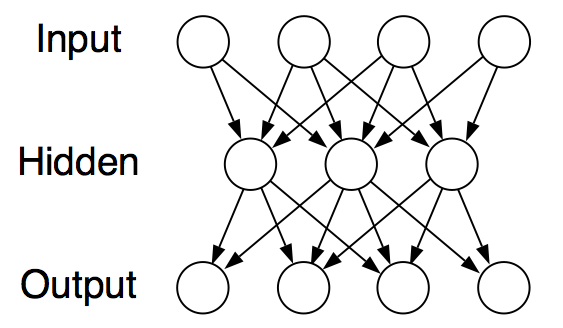
\includegraphics[width=0.6\linewidth]{neural_network}
\captionof{figure}{Feedforward Neural Network\cite{jordan2004introduction}}
\end{center}\vspace{1cm}

Using cross-entropy error ($E$), we can apply backpropagation and optimize the weights and bias terms by stochastic gradient descent using $\frac{\partial E}{\partial W}$, and $\frac{\partial E}{\partial b}$. Much has been written on the classical backpropagation equations so we omit them here, but see \cite{lecun-98b} for an overview. We can then adjust the weights by $\eta \frac{\partial E}{\partial W}$ for some $\eta$, and do the same for the bias terms. Stochastic gradient descent is generally seen as preferable for neural networks given the significant speedups and the ability to escape from local minima so we use that here.\cite{lecun-98b} As some of the input variables are binary indicators, and some are large integers (like age in months), we normalize each input variable such that the mean is $0$ and variance is $0$ so the weights for some the larger valued variables do not dominate the indicator variables. In order to counteract overfitting, we use an early-stopping heuristic to stop training the model when the validation set performance does not improve for a certain number of epochs (100 epochs was a good threshold for this particular problem.) We used the PyBrain library in the implementation, and specified the parameters for the neural network as described above.

\subsection{Experiments}

\begin{center}
% Left or right alignment is specified in the first bracket, the width of the table is in the second
\begin{tabular}{l l l l}
\toprule
\textbf{Dataset} & \textbf{Palocsay et al.} & \textbf{Our results} & \textbf{Naive baseline} \\
\midrule
1978 & 69.20\% (39) & 70.69\% (9) & 64.69\% \\
1980 & 66.98\% (26) & 68.22\% (5) & 62.24\% \\
\bottomrule
\end{tabular}
\captionof{table}{Validation set performance for NN predictor}
\end{center} 

After splitting the 1978 dataset and the 1980 dataset into training and validation sets (7:3 ratio) and training the neural network, validation set performance is improved compared to the results from Palocsay et al \cite{bib1}. The results are also achieved with far fewer nodes in the hidden layer, making it faster to train and likely more generalizable. As the figures below reveal, the neural network starts to quickly overfit as the number of nodes in the hidden layer increases.

\begin{center}\vspace{1cm}
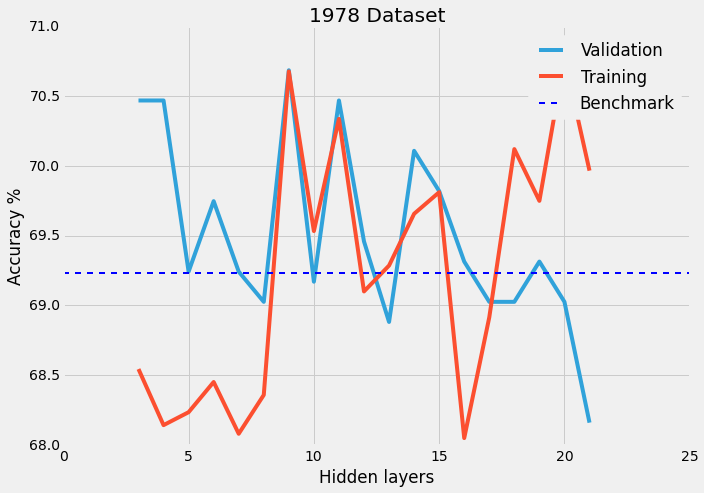
\includegraphics[width=0.9\linewidth]{1978}
\captionof{figure}{1978 Dataset}
\end{center}\vspace{1cm}

\begin{center}\vspace{1cm}
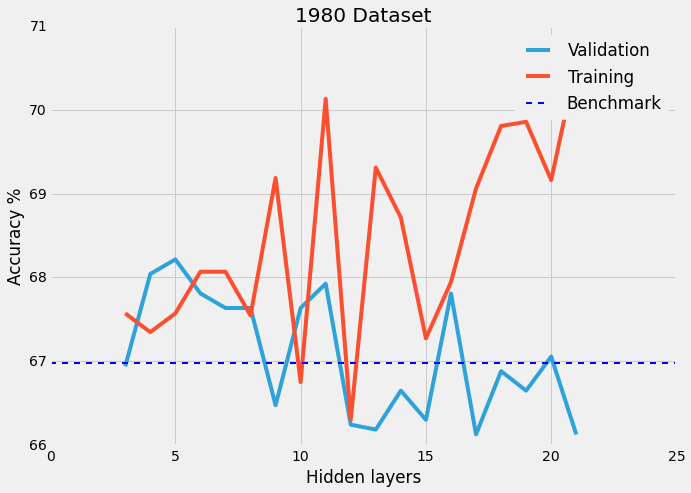
\includegraphics[width=0.9\linewidth]{1980}
\captionof{figure}{1980 Dataset}
\end{center}\vspace{1cm}

\subsection{Discussion}

We also attempted variations such as using a $\tanh$ activation function rather than the logistic function, but the validation set results were notably lower despite recommendations to the contrary \cite{lecun-98b}. We suspect it is something about the nature of the data in this specific problem, but there have been some suggestions that binary classification using $\{-1, 1\}$ rather than $\{0, 1\}$ is better for $\tanh$ activation.\cite{lecun-98b}

\paragraph{}
We attempted to use two hidden layers, but again, validation set results were notably lower likely because even a single hidden layer with a non-linear activation function can approximate significant complexity. Having more than two hidden layers rarely improves performance, and often makes it worse, even though it can theoretically approximate more complex functions. \cite{bengio2007scaling}

\paragraph{}
On the whole, the final configuration worked quite effectively, achieving a substantial improvement over the baseline, and a notable improvement over Pelocsay et al.'s results on the same dataset. In addition, we get better results with far fewer nodes in the hidden layer. Since their paper was from 2000, we believe this improvement is largely due to the strides made around efficient training of neural networks. Now, we can get to very good prediction accuracy with less complexity. Indeed, our experiments to use the same number of nodes as Pelocsay et al. resulted in severe overfitting with poor validation set performance. They also used a proprietary software package with a separate monitoring set used to stop further training so it is difficult to know exactly what other differences there are.

\paragraph{}
As discussed in a later section, the limited information in the dataset is likely making it difficult to get significantly better results; we can hypothesize that recidivism is a very complex topic that is not so easily described by a person's prior background. For example, a person's social circle, the neighborhood they reside in, and situational factors like success in finding a job, all are potential explanatory variables not captured here.\cite{tillyer2011social} We also note that many of profiles had similar backgrounds, but with ultimately different recidivism outcomes, suggesting there is significant relevant information which is not captured in this dataset.

\section{Random Forest}

\subsection{Overview}

In order to get a sense of what features were important in predicting whether a given individual will offend again in the future, we decided to run a random forest. Though the model improved on the base classifier with a score of $67$\% against $62$\%, it did not replicate the performance of the neural network predictor. Our decision to run a random forest was based on their good predictive accuracy (see \cite{caruana2006empirical})

\subsection{Model and Inference}

Remember that our dataset is a collection of records on former convicts. Each entru has 15 features. \textsf{ALCHY} indicates whether the convict has had problem with alcohol, \textsf{MARRIED} their marital status, \textsl{TSERVD} the time served in prison, \textsf{RECID} whether they offend again during the study period - to name a few of them. We are interested in predicting \textsf{RECID}, that is finding a function $f$ such as
$$ \mathsf{RECID} = f(\mathsf{features}) + \mathsf{noise}$$

\paragraph{}
For inference purposes, we consider that the noise is null. The prediction is made on the prediction odds $f(\mathsf{features})$ being greater than a threshold, here $0.5$. The random forest estimator $f$ is actually a sum of decision tree estimator $f_m$. A decision tree is a succession of splits on the dataset. The underlying is to split the data set in different region so that our target variable \textsf{RECID} is constant - or almost constant - in each region. When the split is done, the procedure to predict the label of a new combination of feature is to look at what region it falls into and then attribute the target value in that region (or dominant value).

\begin{figure}[H]
\centering
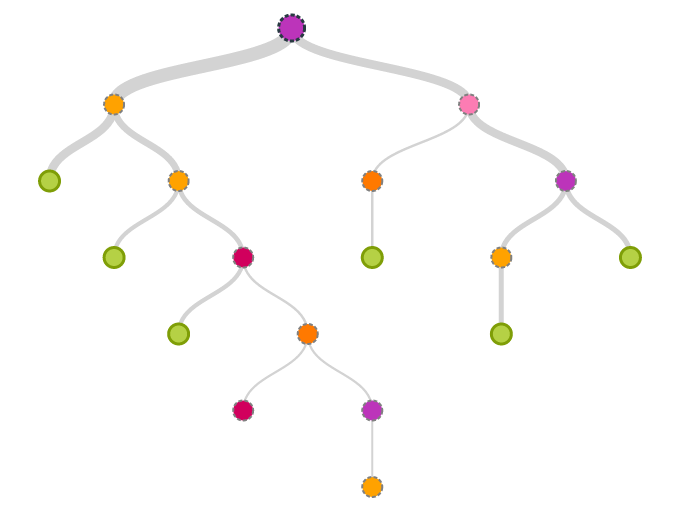
\includegraphics[scale=0.3]{decision_tree.png}
\caption{Decision tree. Each node corresponds to a split of the region into two sub-regions.}
\end{figure}

\subsubsection*{Training a decision tree}

\paragraph{}
To train the decision tree, we grow it with a greedy algorithm - one split at the time. To split the dataset into two or more regions, we choose a feature $x_i$ and condition each region on a specific value of this feature. If $x_i$ is a binary variable, there is a $0-1$ split. If the variable is categorical, we split the region according to the various categories. If the variable is numerical, we look at a $t < x_i$, $t \geq x_i$ split for the feature $x_i$. As for which feature to choose among all the available features, we compute a cost function for each possible split and we choose the combination feature/threshold that has the lowest cost.

\paragraph{}
The cost function is built as follow. Let's name $\mathcal{D}$ the set of all data points that fall in the region we are about to split. Denote by $\pi_0, \pi_1$ the probabilities of a point of $\mathcal{D}$ having respectively label $0$ and label $1$ for \textsf{RECID}.
$$ \pi_0 = \frac{1}{|\mathcal{D}|} \sum_{i \in \mathcal{D}} \mathds{1}_{\mathsf{RECID}_i = 0} \qquad  \pi_1 = \frac{1}{|\mathcal{D}|} \sum_{i \in \mathcal{D}} \mathds{1}_{\mathsf{RECID}_i = 1} $$
In a perfect case, there is only one possibility for the label $\mathsf{RECID}$ and one of these two numbers is $0$. In the worse case, there is a 50-50 split in each of the newly created regions. We tested two functions that measure the purity of the split. The first one was the entropy:

$$H = - \pi_0 \log(\pi_0) - \pi_1 \log(\pi_1) $$
and the second one is the Gini coefficient 
$$ G  = \pi_0(1-\pi_0) + \pi_1(1-\pi_1) $$

\subsubsection*{Training a random forest}

A random forest is an average of decision tree with each tree trained only trained on a subsample of the data and with a subsample of features.

\subsection*{Experiments}

Simulations have shown the cost function's influence on the score of the predictor was not noticeable. The number of feature for each decision tree seems to be located around $5 \sim 6$ and the number of trees around $90$. For each of the figures below, we computed the score of classifiers for various number of trees and various number of features. We define the top score as the classifiers that are in the range $[0.895 * \max \, , \, \max]$ where $\max$ is the score of the best classifier.

\begin{figure}[H]
\centering
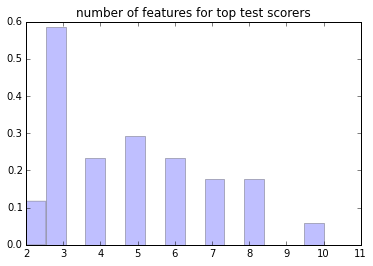
\includegraphics[scale=0.8]{number_features78.png}
\caption{Number of features per tree for the top scorers. 'Gini' loss, $5$ features}
\end{figure}

\begin{figure}[H]
\centering
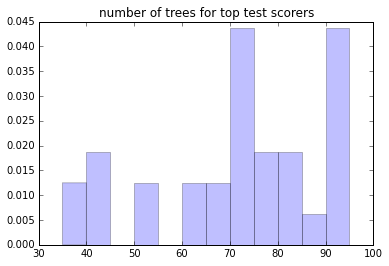
\includegraphics[scale=0.8]{number_forest78.png}
\caption{Number of trees per forest for the top scorers. 'Gini' loss, $100$ trees.}
\end{figure}

We also simulated the impact of the size of the test set. $100$ trees per forest, 'Gini' loss, $5$ features.

\begin{figure}[H]
\centering
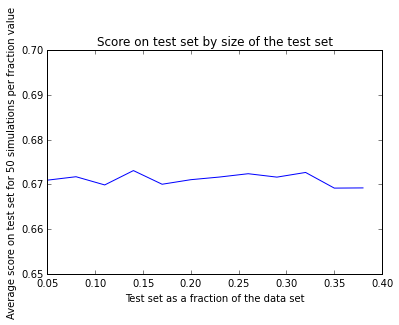
\includegraphics[scale=0.8]{test_size.png}
\caption{Impact of the size of the test set. $100$ trees per forest, 'Gini' loss, $5$ features.}
\end{figure}


\paragraph{}
The most important features for classification are given by the below. A complete description of what is incorporated in each feature can be found at \url{https://www.icpsr.umich.edu/icpsrweb/NACJD/studies/8987?keyword=prison+inmates&permit[0]=AVAILABLE}.


\begin{figure}[H]
\centering
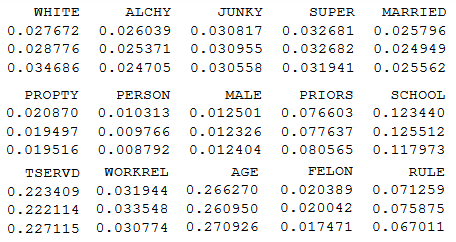
\includegraphics[scale=0.8]{features_weights.png}
\caption{Most important features by frequency of use in the random forest classifier with the best score.}
\end{figure}

\subsection{Remarks on the data}

\paragraph{Score plateau}
The score on the test set seems to have an upper bound at $72$\%, independently of the classification method. One explanation of this plateau is the existence of antagonist duplicates in the data set, that is to say two individuals with very similar features but one is a recidivist and the other is not. Such duplicates would structurally lower the score. The existence of duplicates is made easier by the fact that $13$ of the $16$ feature variable are indicator functions. To address the concern, we looked at the data set. All non-indicator variables were partitioned in groups. For example, the age variable (expressed in months) was replaced with a categorical variable that indicates whether the individual belongs to age group $[0,19], [20, 24], [25,29], [30,34], \dots$. Depending on how we define these groups, we get a duplicate rate between $1$ \% and $10$ \%, which is only a partial explanation for the plateau. Another is simply the lack of data. The $11$ indicator variables represent $2^11 = 2048$ combinations. If we add $5$ non-indicator categorical variables, we get a a number of combinations that is significantly bigger than $9,327$, the number of data points for prisoners released in 1978 or even the total number of data points if we merge the $1978$ and $1980$ files.

\paragraph{Explicative variables}
Random forests classifiers indicate that the number of years spent at school, the age and the duration of the sentence were more important features. This result should be treated cautiously as these three variables happen to be the only 3 variables that are not indicators. Their discriminative power is consequently strengthened.

\section*{Conclusion}

\paragraph{}
We improve upon the existing work done by Palocsay et al. \cite{bib1} on this data set by achieving a higher validation set accuracy using fewer nodes in the hidden layer. The random forest classifiers indicated that the main factors involved in recidivism are the age, the time served in jail and the level of education.

\paragraph{}
A further study of the links between an offender's background, the sentence they receive and the likelihood of recidivism could be studied by incorporating more features and more points. Incorporating more features would reduce the percentage of antagonist points while introducing more points would reduce the complexity of the dataset compared to its size. It seems likely that a neural network would still be the best predictor though some boosting classification algorithm may produce interesting results.

\newpage

\nocite{*}
\bibliographystyle{abbrvnat}
\bibliography{cs281_biblio}

\newpage
\appendix

\section*{Appendix}
\subsection*{A Code for Neural Network}

\begin{lstlisting}
# Get and process input data
import pandas as pd
import numpy as np

var = dict([ (1, ('WHITE',1)),(2, ('ALCHY',1)),(3, ('JUNKY',1)),(4, ('SUPER',1)),
                (5, ('MARRIED',1)),(6, ('FELON',1)),(7, ('WORKREL',1)),(8, ('PROPTY',1)),
                (9, ('PERSON',1)),(10, ('MALE',1)),(11, ('PRIORS',2)),(13, ('SCHOOL',2)),
                (15, ('RULE',2)),(17, ('AGE',3)),(20, ('TSERVD',3)),
                (23, ('FOLLOW',2)),(25, ('RECID',1)),(26, ('TIME',2)),(28, ('FILE',1)) ] )

def cleanData(data):
    res = []
    cols = [x[1][0] for x in var.items()] # Get the column names
    for line in data:
        line = line.strip()
        
        curLine = []
        for i in xrange(len(line)):
            if i+1 not in var:
                continue
            name, sz = var[i+1]            
            curLine.append(int(line[i:i+sz]))
        
        res.append(curLine)
    
    ret = pd.DataFrame(data=res, columns=cols)
    ret = ret[ret.FILE != 3] # Remove incomplete data points
    
    # Remove some irrelevant columns
    del ret['TIME']
    del ret['FILE']
    del ret['FOLLOW']
    return ret
    

raw_1978 = open('data/1978.txt','rb').readlines()
raw_1980 = open('data/1980.txt','rb').readlines()


d1978 = cleanData(raw_1978)
d1980 = cleanData(raw_1980)

print d1978.head()
print len(d1978)

# Neural network for CS 281
# Reference: http://pybrain.org/docs/tutorial

import pybrain
from pybrain.tools.shortcuts import buildNetwork
from pybrain.structure import SoftmaxLayer, TanhLayer
from pybrain.datasets import ClassificationDataSet
from pybrain.supervised.trainers import BackpropTrainer
from pybrain.utilities import percentError
import pickle

def createTrainTest(df, cutProp = 0.3):
    '''
    Input:
        df: Pandas dataframe
        cutProp (default = 0.3): Proportion of samples in the test/validation set
    
    Output:
        trainD: ClassificationDataSet 
        testD: ClassificationDataSet        
    '''
    # Load the dataframe data into the pybrain data set
    np_d1978 = (df.values).astype(float)
    np.random.shuffle(np_d1978)
    cutoff = int(np_d1978.shape[0] * cutProp) # < cutoff is the test set, otherwise training set

    # Normalize
    for c in xrange( np_d1978.shape[1] - 1):
        c_sd = np.std(np_d1978[cutoff:, c])
        c_mean = np.mean(np_d1978[cutoff:, c])

        np_d1978[cutoff:, c] = (np_d1978[cutoff:, c] - c_mean) / c_sd

        # Normalize the test set as well
        np_d1978[:cutoff, c] = (np_d1978[:cutoff, c] - c_mean) / c_sd   

    testD = ClassificationDataSet(np_d1978.shape[1]-1, nb_classes=2, class_labels=['No', 'Yes'])
    trainD = ClassificationDataSet(np_d1978.shape[1]-1, nb_classes=2, class_labels=['No', 'Yes'])    
    

    for r_idx in xrange(len(np_d1978)):
        r = np_d1978[r_idx, :]
        inD, outD = r[:-1], r[-1]

        if r_idx < cutoff:
            testD.appendLinked(inD, outD)
        else:
            trainD.appendLinked(inD, outD)

    # net = buildNetwork(2, 3, 1, hiddenclass=TanhLayer, outclass=SoftmaxLayer)
    trainD._convertToOneOfMany(bounds=[0,1])
    testD._convertToOneOfMany(bounds=[0,1])
    
    return trainD, testD


def findBest(trainD, testD, lower = 3, upper = 26, skip = 1):
    resErr = []

    for hid in xrange(lower, upper, skip):
        print 'Trying with', hid, 'hidden layers...'
        net = buildNetwork(trainD.indim, hid, trainD.outdim, bias=True)
        t = BackpropTrainer(net, dataset=trainD)    

        bestEpoch = None
        bestErr = 101.
        bestTrErr = 101.
        b0Corr = None
        b1Corr = None

        totalIt = 1000
        epPerIt = 10
        maxContinueEpochs = 100

        for it in xrange(totalIt):    
            #     t.trainUntilConvergence(maxEpochs=2000)

            t.trainEpochs(epPerIt)
            testRes = t.testOnClassData(dataset=testD)
            trnresult = percentError( t.testOnClassData(),
                                      trainD['class'] )
            tstresult = percentError( testRes, testD['class'] )

            N1, N0 = 0, 0
            c_1, c_0 = 0, 0
            for i in xrange(len(testRes)):
                if testD['class'][i] == 0:
                    N0 += 1
                    if testRes[i] == 0:
                        c_0 += 1
                else:
                    N1 += 1
                    if testRes[i] == 1:
                        c_1 += 1

            if tstresult < bestErr:
                bestErr = tstresult
                bestTrErr = trnresult
                bestEpoch = t.totalepochs  
                b0Corr = float(c_0)/float(N0)
                b1Corr = float(c_1)/float(N1)

            print 'Prop. of 1s:', sum(testRes)/float(len(testRes))
            print '% of class 0 correct:', float(c_0)/float(N0)
            print '% of class 1 correct:', float(c_1)/float(N1)

            print "epoch: %4d" % t.totalepochs, \
                  "  train acc: %5.2f%%" % (100-trnresult), \
                  "  test acc: %5.2f%%" % (100-tstresult)

            # How long since the last best was found?
            if  t.totalepochs - bestEpoch > maxContinueEpochs:
                print 'Finishing with this cycle; no better scores seen for a while' 
                break

        resErr.append( (bestErr, bestTrErr, hid, bestEpoch, b0Corr, b1Corr, t) )
        print resErr[-1]
    
    return sorted(resErr)


trainD, testD = createTrainTest(d1978)

print trainD.calculateStatistics()
print testD.calculateStatistics()

sRes = findBest(trainD, testD, 3, 22, 1)

print sRes

# Reference: http://stackoverflow.com/questions/6568007/how-do-i-save-and-restore-multiple-variables-in-python
with open('1978_best_trainer.pickle', 'w') as f:
    pickle.dump(sRes[0][-1], f)

with open('1978_res.log', 'w') as f:
    f.write(str(sRes))    
    
    
trainD, testD = createTrainTest(d1980)

print trainD.calculateStatistics()
print testD.calculateStatistics()

sRes = findBest(trainD, testD, 3, 22, 1)

print sRes

# Reference: http://stackoverflow.com/questions/6568007/how-do-i-save-and-restore-multiple-variables-in-python
with open('1980_best_trainer.pickle', 'w') as f:
    pickle.dump(sRes[0][-1], f)

with open('1980_res.log', 'w') as f:
    f.write(str(sRes))

\end{lstlisting}

\subsection*{B Code for Random Forest}

\begin{lstlisting}

get_ipython().magic(u'matplotlib inline')

import pandas as pd
import numpy as np
import matplotlib.pyplot as plt

from __future__ import division

raw_1978 = open('data/1978.txt','rb').readlines()
raw_1980 = open('data/1980.txt','rb').readlines()
d1978 = cleanData(raw_1978)
d1980 = cleanData(raw_1980)


# Baseline Classifier

def baseline(data, target):
    score_baseline_1 = np.size(data[data[target] == 1][target].values) / np.size(data[target].values)
    score_baseline_0 = np.size(data[data[target] == 0][target].values) / np.size(data[target].values)
    print "baseline classifier everyone to 0: ", int(score_baseline_0*100) , "%"
    print "baseline classifier everyone to 1: ", int(score_baseline_1*100) , "%"
    return


baseline(d1978, 'RECID')


# Fit random forest

from sklearn.ensemble import RandomForestClassifier
from sklearn.cross_validation import train_test_split

def score_random_forest(Xtrain, ytrain, Xtest, ytest, n_estimators=10, criterion='gini', max_features='auto'):
    clf= RandomForestClassifier(n_estimators=n_estimators, criterion=criterion, max_features= max_features)
    clf.fit(Xtrain, ytrain)
    score_train = clf.score(Xtrain, ytrain)
    score_test = clf.score(Xtest, ytest)
    return score_train, score_test, clf.feature_importances_

def split(data, list_drop, target, test_size):
    dtrain, dtest = train_test_split(data, test_size = 0.3)
    Xtrain = dtrain.drop(list_drop, axis=1).values
    ytrain = dtrain[target].values
    Xtest = dtest.drop(list_drop, axis=1).values
    ytest = dtest[target].values
    return Xtrain, ytrain, Xtest, ytest   

def best_parameters(Xtrain, ytrain, Xtest, ytest, criterions, nb_trees, nb_features):

    score_tab = pd.DataFrame(columns=['loss', 'nb_trees', 'nb_features', 'test_score', 'train_score', 'features_importance'])
    counter = 0 

    for loss in criterions:
        for n_estimators in nb_trees:
            for max_features in nb_features:
                
                score_train, score_test, features_weights =                 score_random_forest(Xtrain, ytrain, Xtest, ytest, n_estimators=n_estimators, criterion=loss, max_features=max_features) 
                score_tab.loc[counter] = [loss, n_estimators, max_features, score_test, score_train, features_weights]
                counter += 1

    return score_tab

# we wrap everythin inside a sigle function

def classify_random_forest(data, list_drop, target, test_size=0.3, criterions = ['gini'], nb_trees=[10], nb_features = ['auto']):
    Xtrain, ytrain, Xtest, ytest = split(data, list_drop, target, test_size)
    scores =  best_parameters(Xtrain, ytrain, Xtest, ytest, criterions, nb_trees, nb_features)
    return scores

criterions78 = ['gini', 'entropy']
nb_trees78 = np.arange(25,100,5)
nb_features78 = np.arange(1,11)
test_size78 = 0.3

get_ipython().run_cell_magic(u'time', u'', u"scores78 =  classify_random_forest(d1978, ['RECID'], 'RECID', test_size=test_size78, criterions=criterions78, nb_trees=nb_trees78, nb_features=nb_features78)\nprint scores78.head()")

# save file to /data/ folder
file_path = "./data/random_forest_scores78.csv"
scores78.to_json(path_or_buf= file_path)

# recover scores from /data/ folder
#file_path = "./data/random_forest_scores78.csv"
#scores78 = pd.read_json(file_path)
#scores78.head(5)


## Analysis

def relevant_features(scores, threshold = 0.985):
    max_score = np.max(scores.test_score.values)
    print "max score on test set is: ", int(max_score*100), "%"
    
    #extract entries that pass a certain threshold
    winner = scores[scores.test_score > max_score * threshold]
    
    # features used in the selection process
    features_list = pd.DataFrame(columns=['WHITE', 'ALCHY', 'JUNKY', 'SUPER', 'MARRIED', 'FELON',
       'WORKREL', 'PROPTY', 'PERSON', 'MALE', 'PRIORS', 'SCHOOL',
       'RULE', 'AGE', 'TSERVD'])
    
    # create a dataframe with the importance coefficients for each feature
    for i in xrange(len(winner.features_importance.values)):
        features_list.loc[i] = winner.features_importance.values[i]
    
    return features_list, winner.drop('features_importance', axis=1)

features_weights78, top_scorers78 = relevant_features(scores78, threshold = 0.985)
print "we are including in top scores ", int(len(top_scorers78) / len(scores78) * 100) , "% of the sample"
print top_scorers78.head(5)

# we plot a few insightful parameters of the model

plt.title("number of trees for top test scorers")
plt.hist(top_scorers78.nb_trees.values, bins=12, normed=True, color='b', alpha = 0.25)
plt.show()

plt.title("number of features for top test scorers")
plt.hist(top_scorers78.nb_features.values, bins=10, normed=True, color='b', alpha = 0.25)
plt.show()

print features_weights78.head(3)


# ## We adjust the features

X78train_adjusted = d78train.drop(['PERSON', 'RECID', 'FELON', 'PROPTY', 'MALE'], axis=1).values
X78test_adjusted = d78test.drop(['PERSON', 'RECID', 'FELON', 'PROPTY', 'MALE'], axis=1).values
nb_trees_adjusted = np.arange(65,90,2)
nb_features_adjusted = np.arange(4,7)

get_ipython().run_cell_magic(u'time', u'', u'scores_adjusted =  best_parameters(X78train_adjusted, y78train, X78test_adjusted, y78test, criterions, nb_trees_adjusted , nb_features_adjusted)')

features_weights_adjusted, top_scorers_adjusted = relevant_features_adjusted(scores_adjusted, threshold = 0.99)
print "we are including in top scores ", int(len(top_scorers_adjusted) / len(scores_adjusted) * 100) , "% of the sample"
print top_scorers_adjusted.head(5)

plt.title("number of trees for top test scorers with reduced number of features")
plt.hist(top_scorers_adjusted.nb_trees.values, bins=10, normed=True, color='b', alpha = 0.25)
plt.show()

print features_weights_adjusted.head(10)


# 1980 Data set

baseline(d1980, 'RECID')

criterions80 = ['gini', 'entropy']
nb_trees80 = np.arange(25,100,5)
nb_features80 = np.arange(1,11)
test_size80 = 0.3

get_ipython().run_cell_magic(u'time', u'', u"scores80 =  classify_random_forest(d1980, ['RECID'], 'RECID', test_size=test_size80, criterions=criterions80, nb_trees=nb_trees80, nb_features=nb_features80)\nprint scores78.head(5)")

# save file to /data/ folder
file_path = "./data/random_forest_scores80.csv"
scores80.to_json(path_or_buf= file_path)

features_weights80, top_scorers80 = relevant_features(scores80, threshold = 0.985)
print "we are including in top scores ", float(len(top_scorers80)) / len(scores) * 100 , "% of the sample"
print top_scorers80.head(5)

plt.title("number of trees for top test scorers 1980 dataset")
plt.hist(top_scorers80.nb_trees.values, bins=6, normed=True, color='b', alpha = 0.25)
plt.show()

plt.title("number of features for top test scorers 1980 dataset")
plt.hist(top_scorers80.nb_features.values, bins=15, normed=True, color='b', alpha = 0.25)
plt.show()

get_ipython().run_cell_magic(u'time', u'', u'criterions = [\'gini\', \'entropy\']\nnb_trees = np.arange(85,110,5)\nnb_features = [4,5,6]\ntest_size = 0.3\nscores = classify_random_forest(d1980, [\'RECID\'], \'RECID\', test_size=test_size, criterions=criterions, nb_trees=nb_trees, nb_features=nb_features)\n\nfeatures_weights, top_scorers = relevant_features(scores, threshold = 0.985)\nplt.title("number of trees for top test scorers 1980 dataset")\nplt.hist(top_scorers.nb_trees.values, bins=6, normed=True, color=\'b\', alpha = 0.25)\nplt.show()')


# ## Score by size of test set

# We will test 4,5,6 faetures for forest of 100 trees for several variables

def top_test_scores(data, test_try, it = 10, threshold = 0.985, list_drop=['RECID'], target='RECID', criterions = ['gini', 'entropy'], nb_trees=[100], nb_features = [4,5,6]):
    mean_score = []
    mean_features = []
    
    for k in xrange(it):
        scores = classify_random_forest(data, list_drop=list_drop, target=target, test_size=test_try, criterions = criterions, nb_trees=nb_trees, nb_features = nb_features)
        best_score = np.max(scores.test_score.values)
        top_scores = scores[scores.test_score > threshold * best_score].drop('features_importance', axis = 1).head()
        mean_score.append(np.mean(top_scores.test_score))
        mean_features.append(np.mean(top_scores.nb_features))
    
    return np.mean(mean_score), np.mean(mean_features)

def scores_by_test_size(data, test_list, it, threshold = 0.985, list_drop=['RECID'], target='RECID', criterions = ['gini', 'entropy'], nb_trees=[100], nb_features = [4,5,6]):
    score_list = []
    features_list = []
    
    for test_try in test_list:
        mean_score, mean_features = top_test_scores(data, test_try, it, threshold = threshold, list_drop=list_drop, target=target, criterions = criterions, nb_trees=nb_trees, nb_features = nb_features)
        score_list.append(mean_score)
        features_list.append(mean_features)
        print "Done with test set of size: ", test_try, "%"
    
    return score_list, features_list


get_ipython().run_cell_magic(u'time', u'', u'test_list = np.arange(0.05, 0.4 , 0.03)\nscore_list, features_list = scores_by_test_size(d1978, np.arange(0.05, 0.4 , 0.03), 50)')

#we know look at the influence of the test set

import csv

with open('./data/testscore80.csv', 'wb') as myfile:
    wr = csv.writer(myfile, quoting=csv.QUOTE_ALL)
    wr.writerow(score_list)
    
    
with open('./data/featureslist.csv', 'wb') as myfile:
    wr = csv.writer(myfile, quoting=csv.QUOTE_ALL)
    wr.writerow(features_list)

# Score by size of the data set

plt.plot(test_list, score_list)
plt.xlabel("Test set as a fraction of the data set")
plt.ylabel("Average score on test set")
plt.title("Average score on test set by size of the test set for 50 simulations per fraction value")
plt.ylim(0.65,0.70)
plt.show()

# Number of features retained as a size of the data set

plt.plot(test_list, features_list)
plt.xlabel("Test set as a fraction of the data set")
plt.ylabel("Average number of features retained")
plt.title("Average number of features retained by size of the test set for 50 simulations per fraction value")
plt.ylim(4.7,5.2)
plt.show()

\end{lstlisting}

\end{document}